%\documentclass{article}
%\usepackage{amsmath}
%\usepackage{amssymb}
%\usepackage{amsfonts}
%\usepackage{titling}
%\usepackage{graphicx}

%\providecommand{\abs}[1]{\left\vert#1\right\vert}
%\let\vec\mathbf

%\begin{document}

%\title{\textbf{CONSTRUCTION}}
%\date{}
%\maketitle
\begin{enumerate}[label=\thesection.\arabic*.,ref=\thesection.\theenumi]
\numberwithin{equation}{enumi}
\numberwithin{figure}{enumi}
\numberwithin{table}{enumi}



  \item In the given figure, $XZ$ is parallel to $BC$. $AZ$ = 3cm, $ZC$ = 2cm, $BM$ = 3cm and $MC$ = 5cm. Find the length of $XY$.
    \begin{figure}[h!]
      \centering
      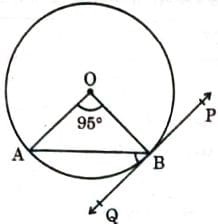
\includegraphics [width=\columnwidth] {figs/fig1.jpg}
      \caption{Isosceles Triangle}
      \label{fig:fig1.jpg}
    \end{figure}

  \item In the given figure, $DE$ $||$ $BC$. If $AD$ = 2units, $DB$ = $AE$ = 3units and $EC$ = $x$units, then find the value of $x$ is:\\

    \begin{figure}[h!]
      \centering
      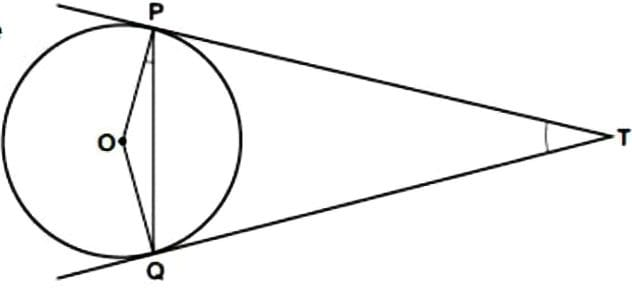
\includegraphics [width=\columnwidth] {figs/fig2.jpg}
      \caption{Right Angle Triangle}
      \label{fig:fig2.jpg}
    \end{figure}

      \begin{enumerate}
        \item 2
        \item 3
        \item 5
        \item $\frac{9}{2}$
      \end{enumerate}

    \newpage

  \item In the given figure, $\Delta ABC$ and $\Delta DBC$ are on te same base $BC$. If $AD$ intersects $BC$ at $\vec{O}$, prove that $\frac { ar(\Delta ABC)}{ar (\Delta DBC)}$ = $\frac{AO}{DO}$.

    \begin{figure}[h!]
      \centering
      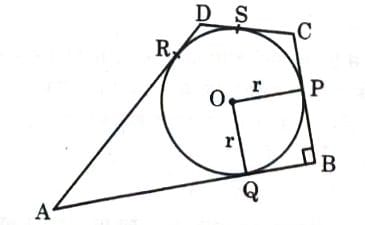
\includegraphics [width=\columnwidth] {figs/fig3.jpg}
      \caption{Triangles with same base}
      \label{fig:fig3.jpg}
    \end{figure}

\end{enumerate}
%\end{document}
